\question به سؤالات زیر پاسخ کامل دهید:

\begin{parts}
    \part[10]  فرض کنید تنها امکان پیاده‌سازی فرآیندهای چندنخی در فضای کاربر (و نه فضای کرنل) مهیاست.
    با این فرض، بزرگ‌ترین مزیت و بزرگ‌ترین عیب چنین پیاده‌سازی از نخ‌ها را چه می‌دانید؟ تحلیل کنید.

    \part[10] با توجه به شکل ۱؛ نمونه درخت فرآیند در سیستم‌عامل لینوکس در اسلاید ۱۰:
    \begin{center}
        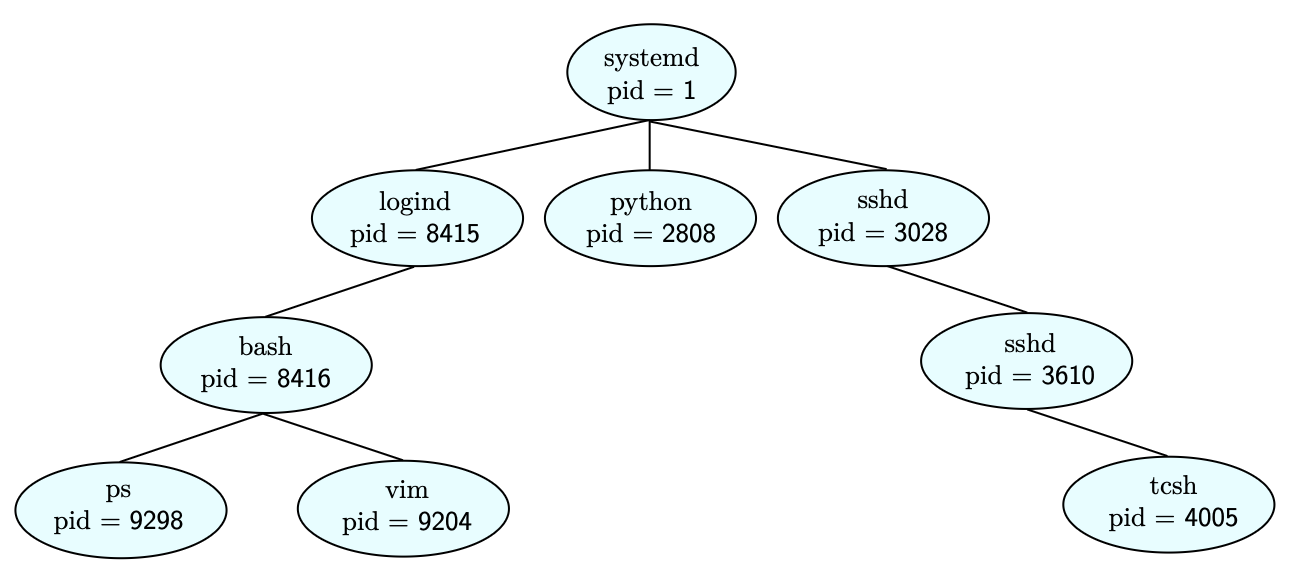
\includegraphics[width=0.8\textwidth]{images/PID_Tree.png}
    \end{center}
    \begin{parts}
        \part در تصویر، چند رابطه‌ی پدر–فرزندی \lr{(Parent–Child Relationship)} وجود دارد؟
        اگر فرآیند {\lr{systemd}} سه فرآیند جدید دیگر ایجاد کند، ساختار درخت چند سطح و چند گره خواهد داشت؟ پاسخ را با تحلیل ساختار فعلی بدهید.

        \part تعداد کل فرآیندها و سطوح درخت را مشخص کنید.
        همچنین بگویید اگر فرآیند {\lr{logind}} خاتمه یابد، دقیقاً چه فرآیندهایی تحت تأثیر قرار می‌گیرند؟
    \end{parts}

    \part[15] در یک سیستم‌عامل فرضی، طراح تصمیم گرفته امکان انتقال یک فرآیند از حالت {\lr{Terminated}} به {\lr{Blocked}} را فراهم کند تا از آن در برخی کاربردهای خاص (مثل بازیابی یا خطایابی) استفاده شود.
    تحلیل کنید که اجرای چنین تصمیمی چه تغییراتی در ساختار سیستم‌عامل و چه چالش‌هایی در زمینه‌ی مدیریت منابع و پایداری فرآیندها به همراه دارد.
    همچنین توضیح دهید در چه شرایطی چنین طراحی می‌تواند موجه یا خطرناک باشد.

\end{parts}